% % Created 2015-09-15 Tue 11:46
% \documentclass[11pt]{article}
% \usepackage[utf8]{inputenc}
% \usepackage[T1]{fontenc}
% \usepackage{fixltx2e}
% \usepackage{graphicx}
% \usepackage{longtable}
% \usepackage{float}
% \usepackage{wrapfig}
% \usepackage{rotating}
% \usepackage[normalem]{ulem}
% \usepackage{amsmath}
% \usepackage{textcomp}
% \usepackage{marvosym}
% \usepackage{wasysym}
% \usepackage{amssymb}
% \usepackage{hyperref}
% \usepackage{color}
% \usepackage{soul}
% \tolerance=1000
% \usepackage[margin=1in]{geometry}

% \newcommand{\hilight}[1]{\colorbox{yellow}{#1}}


%\begin{document}
\section{Body Extender}
\label{bodyExtender}
\begin{refsection}[exos/bodyExt.bib]

The Body Extender is one of the few existing full-body exoskeletons.  The Body Extender's main objective is to increase the forceful interaction capabilities, specifically the heavy load handling capabilities, of an operator in difficult and unknown environments.  The overall suit is composed of four robotic limbs with kinematics designed to be anthropomorphically similar.  The suit contains twenty-two independently actuated degrees of freedom.  Note that the Body Extender is the only fully actuated suit included in this report.  The fully actuated design of the suit was chosen based on the fact that handling, or rather manipulating heavy objects requires forces and torques that far exceed human capabilities.  Note also that having many actuated degrees of freedom means that fully actuated suits will be very heavy, and thus will require specialized controllers.

As a primary objective, the Body Extender aims to allow operators to use the hardware with minimal training.  Thus, the system is designed so as not to require substantial modifications to human motor habits.  The effective mass distribution of the suit, of special consideration in these heavy systems, is designed to be similar to that of an unloaded operator.  Like most other strength augmentation exoskeletons, the Body Extender is intended to minimize resistive forces between the operator and suit, even when the suit is not loaded externally. 

A picture of the Body Extender exoskeleton and its five main components, four limbs and a torso, is shown in Figure \ref{fig:bodyExt}.
\begin{figure}[thpb]
\centering
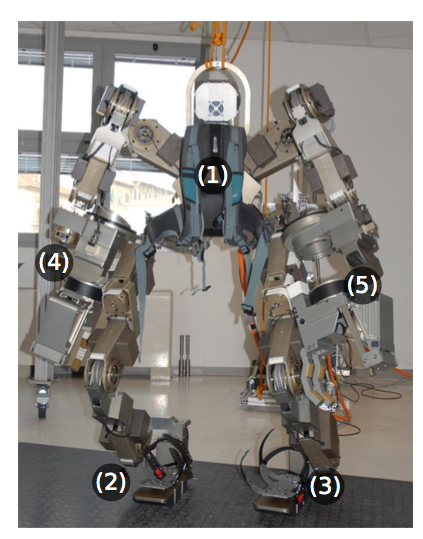
\includegraphics[width=3.in]{exos/figs/bodyExt/bodyExt}
  \caption{The Body Extender.}
%  \vspace{-0.2in}
 \label{fig:bodyExt}   
 \end{figure}
 

\subsection{Actuator Specifications}
 
 Except for forearm pronosupination, each of the actuators in the Body Extender suit are driven by a linear actuator that is composed of an electrical motor, incremental encoder, ball screw, and angular contact ball bearings.  The motors are frame-less DC torque controlled motors.  The {\bf peak torque of the motors is 7 Nm, with a maximum continuous torque of 6 Nm}.  Each motor weighs 1.4 kg.  The {\bf linear actuator assembly is able to supply 8000 N with a total weight of 2.4 kg}.
 
 Joints that have a small range of motion and low torque requirements use linear actuators in straightforward lever mechanism configurations.  For degrees of freedom which require relatively large ranges of motion as well as torque, a motion conversion system transforms the linear actuator motion into rotational motion.  The motion conversion unit consists of a pantograph, two metallic tendons, and an output pulley connected to the output link.  A CAD drawing of the motion conversion unit is shown in Figure \ref{fig:motionConv}. 
 \begin{figure}[thpb]
\centering
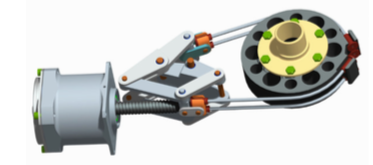
\includegraphics[width=3.in]{exos/figs/bodyExt/motionConv}
  \caption{CAD view of the internal components of the actuation module.}
%  \vspace{-0.2in}
 \label{fig:motionConv}   
 \end{figure}
 There are two configurations of the motion conversion unit.  The first has a {\bf maximum continuous output of 500 Nm and the second a maximum continuous output of 270 Nm}.  The two units weigh 6 kg and 5 kg respectively, and have {\bf mechanical efficiency of about 85\%}.  {\bf The speed of the actuators is approximately 60 deg/s}.
 
 
 \subsection{Exoskeleton Specifications}
 
 The Body Extender's twenty-two actuated degrees of freedom include two arms, two legs, and a torso or central backpack unit.   The arms have a servo-amplified degree of freedom for grasping heavy objects.  Grasping forces are achieved using a force sensing trigger mechanism; the force is proportional to the force applied to the trigger.
 
 The suit contains twenty-two incremental encoders that measure angular displacement of each of the electric motors.  There are also {\bf five six-axis force/torque sensors mounted at the five connecting points between the user and the device; two at the hands, two at the feet, and one on the trunk.}  These sensors directly measure the forces and torques between the user and the suit.  There are additionally two single axis force sensors integrated into the grippers that measure the force applied by the operator on the ``gripper triggers," as well as {\bf a three axis accelerometer integrated into the backpack unit which estimates the trunk orientation}.  Lastly, \textbf{accelerometers are distributed throughout the system} to monitor link dynamics, supporting overall equilibrium and internal stability during manipulation tasks.   
 
{\bf The control software is distributed between a central processing unit and sixteen local units located throughout the system}.  The communication between processing units is handled using a high-speed field bus.
 
{\bf The system is powered using thirteen batteries in series, which provide a nominal voltage of 78 V}.  When the system is run in stand-alone mode, the batteries can provide eight hours of continuous work.
 
 
 \subsection{Control Specifications}
 
 The body extender control algorithm centers around a {\bf feedback linearization policy} that depends on measuring the force between the operator and suit, knowing the contact state of the suit and environment, decoupling the control of each of the limbs for each other, and having each limb be fully actuated.  The dynamics for each of the Body Extender limbs are written in standard form as  
\begin{equation}
\mB_i(q) \ddot{q} + \mC_i(q,\dot{q})\dot{q} + \mG_i(q) = {\bf \tau} + \mJ^T_{iu}{\bf F_s} + \mJ^T_{ia}{\bf F_a},
\end{equation}
where $i$ is an integer corresponding to a different limb, ${\bf \tau}$ represents the actuator torques, ${\bf F_s}$ the measured forces between the operator and suit, and ${\bf F_a}$ the unmeasured contact forces on the suit.  The $\mB_i$, $\mC_i$, and $\mG_i$ terms represent the limb inertia, Coriolis and centrifugal, and gravitational torques.  

The authors in \cite{body_control_2012} use a decoupling strategy in their controllers which enables the individual limbs in the Body Extender to be somewhat decoupled from each other.  They claim that they accomplish this using the following model:
\begin{equation}
\mB_i(q) \ddot{q} + \mC_i(q,\dot{q})\dot{q} + \mG_{iT}(q) = {\bf \tau} + \mJ^T_{iu}F_s + \mJ^T_{ia}F_a - \mB_{iT}{q}\dot{V}_T - \mC_{iT}(q,\dot{q}){\bf V_T},
\end{equation}
where, ${\bf V_T}$ is the trunk velocity, $\mG_{iT}$ the gravitational effect of the trunk on the limb, $\mB_{iT}$ the inertia of the trunk acting on the limb, and $\mC_{iT}$ the trunk Coriolis and centrifugal term.  Note that ${\bf V_T}$ and $\dot{{\bf V}}_{\bf T}$ are directly measured through the accelerometer and gyroscope in the trunk.

The feedback linearizing controller in \cite{} operates under two fundamental assumptions and only appears to relate directly to the case of a single manipulator arm.  The first assumption of the controller is that the mass and inertial properties of an object being manipulated are estimated online.  The second is that the forces measured between the operator and suit can be modeled as
\begin{equation}
\vF_s = \mM_p \dot{\vV}_e + \vG_p,
\label{eq:forceEq}
\end{equation}
where $\mM_p$ is an effective mass of the end effector, $\dot{\vV}_e$ is the acceleration of the end effector, and $\mG_p$ is an effective gravitational term.  Note that the gravitational term is zero if the arm is not holding an external load.  The importance of these two assumptions will be more clear after the analytical forms of the feedback linearizing controllers are introduced. 

The dynamics of the arm when not manipulating a load are
\begin{equation}
\mB(\vq) \ddot{\vq} + \mC(\vq,\dot{\vq})\dot{\vq} + \mG(\vq) = {\bf \tau}. \notag
\end{equation} 
The feedback linearizing controller for this case has the form
\begin{equation}
{\bf \tau} = \mB(\vq)(\ddot{\vq}_d + K_v \dot{\tilde{\vq}} + K_p \tilde{\vq}) + \mC(\vq,\dot{\vq})\dot{\vq} + \mG(\vq), \notag
\end{equation}
where $\tilde{\vq} = \vq_d - \vq$.  The details are unclear in \cite{body_control_2012}, but it appears that the authors either propose using predefined trajectories to define $\ddot{\vq}_d$, $\dot{\vq}_d$, and $\vq_d$, or use the assumption in \eqref{eq:forceEq} to determine these values.  
%\begin{equation}
%\vF_s = \mM_p \dot{V}_e
%\label{eq:assump1}
%\end{equation}
Equation \ref{eq:forceEq} relates the measured force to the derivative of the end effector velocity $\dot{\vV}_e$.  This end effector velocity can then be related to the desired joint velocities using the analytical Jacobian transformation \[ \ddot{\vq}_d = \mJ(\vq)^{-1}(\dot{V}_e - \dot{J}(\vq,\dot{\vq})\dot{\vq}).\]  The values for $\dot{\vq}_d$ and $\vq_d$ can then be found through integration.  It is not clear the how authors explicitly decouple the human dynamics from the robot in this case.

In the case where the exoskeleton arm is manipulating a load, the feedback linearizing controller has the augmented form
\begin{equation}
{\bf \tau} = \mB(\vq)(\ddot{\vq}_d + K_v \dot{\tilde{\vq}} + K_p \tilde{\vq}) + \mC(\vq,\dot{\vq})\dot{\vq} + \mG(\vq) -\mJ^T(\vq) \vF_s -\mJ^T(\vq)\vF_a. \notag
\end{equation}
The main difference in this case is that the controller here explicitly compensates for the measured human-robot interaction force $\vF_s$, and the controller includes the un-sensed forces $\vF_a$ which arise from the object being manipulated.  The object interaction forces thus need to be estimated.  The ability to estimate these forces is the first fundamental assumption on which the Body Extender's control scheme relies.  Because the point at which the manipulator arm and object are connected is assumed to be well known, and the arm is instrumented with inertial sensors, estimating the interaction forces of the manipulated object is be assumed to be equivalent to estimating its inertial properties.  As outlined in \cite{body_control_2012}, this is accomplished using a standard regressor which uses the input and output of the feedback linearizing controller as the basis for the regression.  The details of this process are left to \cite{body_control_2012}.

 
\subsection{Assessment and Recommendations}

The Body Extender suit is one of the only fully-actuated upper and lower extremity exoskeletons available today.  Clearly, for the task of handling extremely heavy objects, a fully actuated suit may be the best option, but, generally speaking, having the addition weight due to actuating every degree of freedom in the suit is not ideal when considering dynamic operation.  

The controllers highlighted in \cite{body_control_2012} do present some novel components.  For example, using a regressor to estimate unknown external forces may be an idea which is directly applicable to a variety of different projects.  Note that in the case of the Body Extender, this regression is dependent on knowing the location of the external force relative to the suit, the manipulator end effectors.  Thus, an extension of this idea, possibly using a lager distribution of sensors to measure external forces, is necessary to extend this approach more generally.  

The way that the Body Extender control uses operator-robot measured interaction forces to generate desired trajectories around which a stabilizing controller is designed is generally an idea that we support.  Note that, like any of the model-based control approaches outlined in the exoskeleton literature the feedback linearizing controller in this work is dependent on knowing the model of the robot hardware with a relatively high-level of fidelity.  

In terms of the controlling of the overall suit, i.e., locomotion in addition to manipulation, it was difficult to find any papers that discussed more than upper-body single-arm control of a manipulated object for the Body Extender hardware.  The stated strategy of decoupling the individual limbs from each other seems somewhat feasible, but is limited relative to coordinated limb control. 

 The mechanical specifications as well as figures related to mechanical design for the Body Extender system discussed in this section are based on and taken from \cite{body_design_2011}.  The discussion of the control system is based on work presented in \cite{body_control_2012}.

\printbibliography[heading=subbibliography]

\end{refsection}
  
% \end{document}


% S. Marcheschi, F. Salsedo, M. Fontana, and M. Bergamasco, Body Extender: Whole body exoskeleton for human power augmentation, in Proc. IEEE Int. Conf. Robotics Automation, 2011, pp. 611?616.


% G.P. Rosati Papini, and C.A. Avizzano, "Transparent Force Control for Body Extender," 2012 IEEE RO-MAN: The 21st IEEE International Symposium on Robot and Human Interactive Communication, 2012, pp. 138-143.




%%% Local Variables:
%%% mode: latex
%%% TeX-master: "../survey"
%%% End:
